\documentclass{article}
\usepackage{graphicx}
\usepackage{booktabs} % for \toprule, \midrule, and \bottomrule

\begin{document}
	
	\begin{figure}[h]
		\centering
		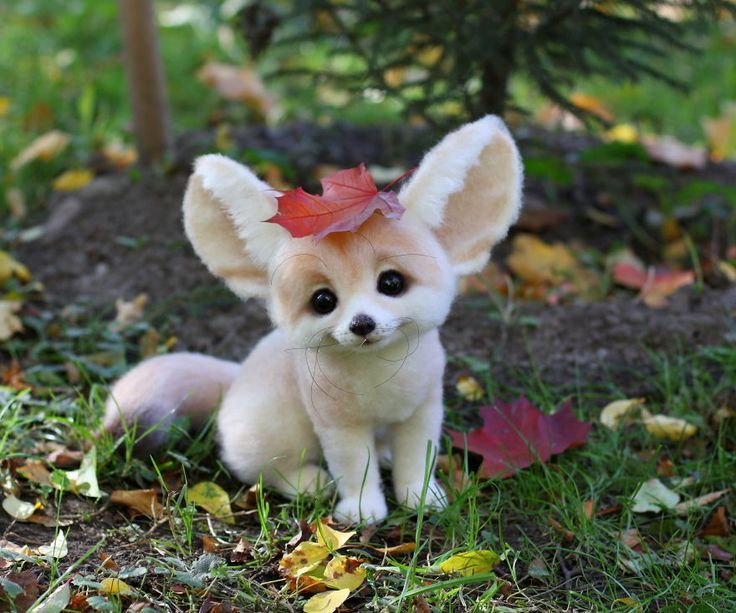
\includegraphics[width=\linewidth]{cute.jpeg}
		\caption{Example image}
	\end{figure}
	

	
\begin{table}
	\label{table}
	\centering
	\caption{Student Data}
	\begin{tabular}{c|c|c|c|c}
		\hline
		\textbf{Mis}& \textbf{Name}&\textbf{Gender} &\textbf{Branch}& \textbf{Class} \\
		\hline
		112101054 & Prathmesh & Male & Civil & Fy btech\\
		\hline
		112103025 & Paras & Male & Computer & Fy btech\\
		\hline
		11210124 & Swayam & Male & Mechanical & Fy btech\\
		\hline
		112103026 & Yash & Male & Computer & Fy btech\\
		\hline
		11203034 & Harshvardhan & Male & Computer & Fy btech\\
		\hline
		112102034 & Aditya & Male & Civil & Fy btech\\
		\hline
		112105036 & Sumit & Male & Electrical & Fy btech\\
		\hline
		112104038 & Sai & Female & IT & Fy btech\\
		\hline
		112103126 & Digvijay & Male & Computer & Fy btech\\
	\end{tabular}
\end{table}
	
\end{document}
